\documentclass[tikz]{standalone}

\usepackage[utf8]{inputenc}
\usepackage[T1]{fontenc}

\usetikzlibrary{math}


\begin{document}
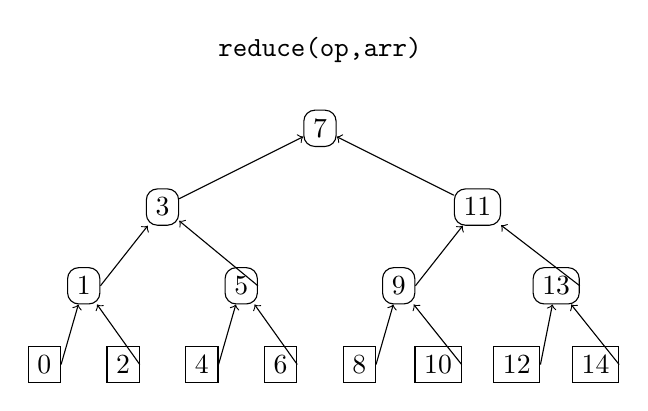
\begin{tikzpicture}[
  scale=0.5,
  array_element/.style={
    draw
  },
  reduced_array_element/.style={
    draw,rounded corners
  }]
  %
  \foreach \x in {0,2,...,14} {
    \node[array_element] (arr_\x) at (\x,0) {\x};
  }
  \foreach \z in {1,5,...,13} {
    \node[reduced_array_element] (l1_\z) at (\z,2) {\z};
    \tikzmath {
      \x = \z - 1;
      \y = \z + 1;
    }
    \draw[->] (arr_\x) -- (l1_\z);
    \draw[->] (arr_\y) -- (l1_\z);
  }
  \foreach \z in {3,11} {
    \node[reduced_array_element] (l2_\z) at (\z,4) {\z};
    \tikzmath {
      \x = \z - 2;
      \y = \z + 2;
    }
    \draw[->] (l1_\x) -- (l2_\z);
    \draw[->] (l1_\y) -- (l2_\z);
  }
  \node[reduced_array_element] (l3_7) at (7,6) {7};
  \draw[->] (l2_3) -- (l3_7);
  \draw[->] (l2_11) -- (l3_7);
  %
  \node at (7,8) {\texttt{reduce(op,arr)}};
\end{tikzpicture}
\end{document}


% vim: set sw=2 sts=2 et :
